%Version 3 October 2023
% See section 11 of the User Manual for version history
%
%%%%%%%%%%%%%%%%%%%%%%%%%%%%%%%%%%%%%%%%%%%%%%%%%%%%%%%%%%%%%%%%%%%%%%
%%                                                                 %%
%% Please do not use \input{...} to include other tex files.       %%
%% Submit your LaTeX manuscript as one .tex document.              %%
%%                                                                 %%
%% All additional figures and files should be attached             %%
%% separately and not embedded in the \TeX\ document itself.       %%
%%                                                                 %%
%%%%%%%%%%%%%%%%%%%%%%%%%%%%%%%%%%%%%%%%%%%%%%%%%%%%%%%%%%%%%%%%%%%%%

%%\documentclass[referee,sn-basic]{sn-jnl}% referee option is meant for double line spacing

%%=======================================================%%
%% to print line numbers in the margin use lineno option %%
%%=======================================================%%

%%\documentclass[lineno,sn-basic]{sn-jnl}% Basic Springer Nature Reference Style/Chemistry Reference Style

%%======================================================%%
%% to compile with pdflatex/xelatex use pdflatex option %%
%%======================================================%%

%%\documentclass[pdflatex,sn-basic]{sn-jnl}% Basic Springer Nature Reference Style/Chemistry Reference Style


%%Note: the following reference styles support Namedate and Numbered referencing. By default the style follows the most common style. To switch between the options you can add or remove “Numbered” in the optional parenthesis. 
%%The option is available for: sn-basic.bst, sn-vancouver.bst, sn-chicago.bst%  
 
%%\documentclass[sn-nature]{sn-jnl}% Style for submissions to Nature Portfolio journals
%%\documentclass[sn-basic]{sn-jnl}% Basic Springer Nature Reference Style/Chemistry Reference Style
%%%%\documentclass[sn-mathphys-num]{sn-jnl}% Math and Physical Sciences Numbered Reference Style 
%%\documentclass[sn-mathphys-ay]{sn-jnl}% Math and Physical Sciences Author Year Reference Style
%%\documentclass[sn-aps]{sn-jnl}% American Physical Society (APS) Reference Style
%%\documentclass[sn-vancouver,Numbered]{sn-jnl}% Vancouver Reference Style
%%\documentclass[sn-apa]{sn-jnl}% APA Reference Style 
%%\documentclass[sn-chicago]{sn-jnl}% Chicago-based Humanities Reference Style

\let\LaTeXcline\cline\documentclass[sn-mathphys-num]{sn-jnl}\let\cline\LaTeXcline

%%%% Standard Packages
%%<additional latex packages if required can be included here>

\usepackage{graphicx}%
\usepackage{multirow}%
\usepackage{amsmath,amssymb,amsfonts}%
\usepackage{amsthm}%
\usepackage{mathrsfs}%
\usepackage[title]{appendix}%
\usepackage{xcolor}%
\usepackage{textcomp}%
\usepackage{manyfoot}%
\usepackage{booktabs}%
\usepackage{algorithm}%
\usepackage{algorithmicx}%
\usepackage{algpseudocode}%
\usepackage{listings}%
%%%%
\usepackage{anyfontsize}

%%%%%=============================================================================%%%%
%%%%  Remarks: This template is provided to aid authors with the preparation
%%%%  of original research articles intended for submission to journals published 
%%%%  by Springer Nature. The guidance has been prepared in partnership with 
%%%%  production teams to conform to Springer Nature technical requirements. 
%%%%  Editorial and presentation requirements differ among journal portfolios and 
%%%%  research disciplines. You may find sections in this template are irrelevant 
%%%%  to your work and are empowered to omit any such section if allowed by the 
%%%%  journal you intend to submit to. The submission guidelines and policies 
%%%%  of the journal take precedence. A detailed User Manual is available in the 
%%%%  template package for technical guidance.
%%%%%=============================================================================%%%%

%% as per the requirement new theorem styles can be included as shown below
%\theoremstyle{thmstyleone}%
\newtheorem{theorem}{Theorem}%  meant for continuous numbers
%%\newtheorem{theorem}{Theorem}[section]% meant for sectionwise numbers
%% optional argument [theorem] produces theorem numbering sequence instead of independent numbers for Proposition
\newtheorem{proposition}[theorem]{Proposition}% 
%%\newtheorem{proposition}{Proposition}% to get separate numbers for theorem and proposition etc.

%\theoremstyle{thmstyletwo}%
\newtheorem{example}{Example}%
\newtheorem{remark}{Remark}%

%\theoremstyle{thmstylethree}%
\newtheorem{definition}{Definition}%

\raggedbottom
%%\unnumbered% uncomment this for unnumbered level heads

\usepackage[acronym]{glossaries}
\renewcommand{\glstextformat}[1]{\color{black}#1}

\makeglossaries
\newacronym{doi}{DOI}{Digital Object Identifier}
\newacronym{dst}{Dst}{Disturbance Storm-Time}
\newacronym{rin}{RIN}{The Royal Institute of Navigation}
\newacronym{ion}{ION}{The Institute of Navigation}
\newacronym{ursi}{URSI}{Union Radio-Scientifique Internationale}
\newacronym{rinex}{RINEX}{Receiver Independent Exchange Format}
\newacronym{tec}{TEC}{Total Electron Content}
\newacronym{dtec}{dTEC}{standard deviation of Total Electron Content}
\newacronym{gnss}{GNSS}{Global Navigation Satellite System}
\newacronym{pnt}{PNT}{Positioning, Navigation, and Timing}
\newacronym{svm}{SVM}{Support Vector Machine}
\newacronym{svn}{SVN}{Support Vector Network}
\newacronym{dt}{DT}{Decision Tree}
\newacronym{tdidt}{TDIDT}{Top-Down Induction of Decision Trees}
\newacronym{nb}{NB}{Naive Bayes}
\newacronym{ci}{CI}{Confidence Interval}
\newacronym{nir}{NIR}{No Information Rate}
\newacronym{nn}{NN}{Neural Network}
\newacronym{ann}{ANN}{Artificial Neural Network}
\newacronym{pls}{PLS}{Partial Least Squares}
\newacronym{pls-da}{PLS-DA}{Partial Least Squares Discriminant Analysis}
\newacronym{fda}{FDA}{Flexible Discriminant Analysis}
\newacronym{lda}{LDA}{Linear Discriminant Analysis}
\newacronym{pca}{PCA}{Principal Component Analysis}
\newacronym{manova}{MANOVA}{Multivariate Analysis Of Variance}
\newacronym{mars}{MARS}{Multivariate Adaptive Regression Splines}
\newacronym{nda}{NDA}{Normal Discriminant Analysis}
\newacronym{nas}{NAS}{Neural Architecture Search}
\newacronym{dbscan}{DBSCAN}{Density-Based Spatial Clustering}
\newacronym{cnn}{CNN}{Convolutional Neural Network}
\newacronym{rf}{RF}{Random Forest}
\newacronym{tp}{TP}{True Positive}
\newacronym{tn}{TN}{True Negative}
\newacronym{fp}{FP}{False Positive}
\newacronym{fn}{FN}{False Negative}
\newacronym{tpr}{TPR}{True Positive Rate}
\newacronym{tnr}{TNR}{True Negative Rate}
\newacronym{ppv}{PPV}{Positive Predictive Value}
\newacronym{npv}{NPV}{Negative Predictive Value}
\newacronym{dr}{DR}{Detection Rate}
\newacronym{dp}{DP}{Detection Prevalence}
\newacronym{ba}{BA}{Balanced Accuracy}
\newacronym{sar}{SAR}{Synthetic Aperture Radar}
\newacronym{cca}{CCA}{Canonical Correlation Analysis}
\newacronym{pod}{POD}{Proper Orthogonal Decomposition}
\newacronym{svd}{SVD}{Singular Value Decomposition}
\newacronym{eof}{EOF}{Empirical Orthogonal Functions}
\newacronym{evd}{EVD}{Eigenvalue Decomposition}
\newacronym{gps}{GPS}{Global Positioning System}
\newacronym{klt}{KLT}{Karhunen–Loève Theorem}
\newacronym{gpu}{GPU}{Graphics Processing Unit}
\newacronym{cpu}{CPU}{Central Processing Unit}
\newacronym{ram}{RAM}{Random Access Memory}
\newacronym{ml}{ML}{machine learning}
\newacronym{aa2}{(AA)2}{Ambient-Aware Application-Aligned}
\newacronym{tid}{TID}{Traveling Ionospheric Disturbance}
\newacronym{epb}{EPB}{Equatorial Plasma Bubbles}
\newacronym{gec}{GEC}{Global Electric Current}
\newacronym{spdf}{SPDF}{Space Physics Data Facility}
\newacronym{noaa}{NOAA}{National Oceanic and Atmospheric Administration}
\newacronym{swpc}{SWPC}{Space Weather Prediction Center}
\newacronym{nrcan}{NRCAN}{Natural Resources Canada}
\newacronym{gfz}{GFZ}{German Research Centre for Geosciences}
\newacronym{nasa}{NASA}{National Aeronautics and Space Administration}
\newacronym{euv}{EUV}{Extreme ultraviolet}

\renewcommand*{\acronymname}{List of abbreviations} 

\begin{document}

\title[A $Dst$-based space weather conditions machine learning classification model for GNSS PNT performance analysis]{A $Dst$-based space weather conditions machine learning classification model for GNSS PNT performance analysis}

\author*[1,2]{\fnm{Lucija} \sur{\v{Z}u\v{z}i\'{c}}}\email{lucija.zuzic@uniri.hr}
\equalcont{These authors contributed equally to this work.}

\author[1,2]{\fnm{Deni} \sur{Klen}}\email{deni.klen@uniri.hr}

\author[3]{\fnm{Teodor B.} \sur{Iliev}}\email{tiliev@uni-ruse.bg}

\author[1,2,4]{\fnm{Renato} \sur{Filjar}}\email{renato.filjar@uniri.hr}

\affil*[1]{\orgdiv{Department of Computer Engineering}, \orgname{Faculty of Engineering, University of Rijeka}, \orgaddress{\street{Vukovarska 58}, \city{Rijeka}, \postcode{51000}, \country{Croatia}}}

\affil[2]{\orgdiv{Center for Artificial Intelligence and Cybersecurity}, \orgname{University of Rijeka}, \orgaddress{\street{Radmile Matejcic 2}, \city{Rijeka}, \postcode{51000}, \country{Croatia}}}

\affil[3]{\orgdiv{Department of Telecommunication}, \orgname{University of Ruse}, \orgaddress{\street{8 Studentska str.}, \city{Ruse}, \postcode{7017}, \country{Bulgaria}}}

\affil[4]{\orgdiv{Laboratory for Spatial Intelligence}, \orgname{Hrvatsko Zagorje Krapina University of Applied Sciences}, \orgaddress{\street{Setaliste hrvatskog narodnog preporoda 6}, \city{Krapina}, \postcode{49000}, \country{Croatia}}}

\abstract{Ambient conditions classification enables systematic mitigation of adversarial effects on Global Navigation Satellite System (GNSS) Positioning, Navigation, and Timing (PNT) performance. This research contributes to the problem by proposing a classification model of space weather events for sub-equatorial regions. The proposed model uses machine learning-based classification applied to the experimental observations of geomagnetic field components, observed Total Electron Content ($TEC$), and Disturbance Storm-Time ($Dst$-index). A Support Vector Machine (SVM) with a Polynomial Kernel, C5.0 Decision Tree (DT), Naive Bayes (NB), shallow Neural Network (NN), Partial Least Squares (PLS), Flexible Discriminant Analysis (FDA), and shallow NN using Principal Component Analysis (PCA) was applied to develop the candidate model to classify observations of the geomagnetic field in $TEC$, combined with other variables, into one of the scenarios of space weather conditions. Performance is assessed using a confusion matrix and development time to yield the NB as the best performer. The proposed $Dst$-based classification model serves as an indicator of a geomagnetic/ionospheric storm in progress, thus alerting GNSS users of potential degradation in GNSS PNT performance and setting up a framework for the development of a tailored GNSS ionospheric correction model for specific classes of the space weather conditions.}

\keywords{Global Navigation Satellite System (GNSS) Positioning, Navigation, and Timing (PNT), space weather conditions, machine learning (ML), classification model, Decision Tree (DT), Neural Network (NN), sensor observations aggregation, geomagnetic field, Total Electron Content ($TEC$), Disturbance Storm-Time ($Dst$-index)}

%%\pacs[JEL Classification]{D8, H51}

%%\pacs[MSC Classification]{35A01, 65L10, 65L12, 65L20, 65L70}

\maketitle

\section{Introduction}
%\label{sec:Intro}

The Global Navigation Satellite System (GNSS) and its Positioning, Navigation, and Timing (PNT) service have matured to become an essential part of national infrastructure, public goods, and enablers of a vast number of emerging technology and socio-economic applications citestuff(spilker1996global). Maintaining the GNSS PNT quality is crucial for the sustainable development of modern economy and society citestuff(schaer1999mapping). Overcoming the shortcomings and vulnerabilities of GNSS PNT is a scientific challenge, and the need of a wide variety of scientists, developers, operators, regulators, and users of GNSS-based systems and services citestuff(durmaz2015regional, jin2012m_dcb). The Earth’s ionosphere, a part of the Earth’s atmosphere stretching from $50$ $km$ to $2000$ $km$ above the Earth’s surface and comprised of rare but mostly charged atoms and molecules, is the major natural cause of GNSS PNT degradation citestuff(davies1990ionospheric, liu2009seismoionospheric). This phenomenon especially affects most currently used GNSS receivers, which work as single-frequency receivers exposed to GNSS ionospheric effects citestuff(spilker1996global, prolss2012physics). Driven by powerful and random flows of energy and particles from the Sun (space weather conditions), the ionospheric conditions define the properties of GNSS signal propagation through the Earth’s atmosphere and the resulting ionospheric delay citestuff(davies1990ionospheric, oxley2017uncertainties, prolss2012physics). The GNSS ionospheric delay causes errors in GNSS PNT algorithm deployment, designed to produce position, velocity, and time estimates for a GNSS receiver citestuff(spilker1996global, schaer1999mapping). The ionosphere affects GNSS satellite signals for position estimation by introducing signal propagation delay citestuff(spilker1996global, schaer1999mapping). The GNSS ionospheric delay is a stochastic variable, whose value is determined by complex physical processes of space weather citestuff(spilker1996global, schaer1999mapping). How space weather affects GNSS PNT performance was explained using the Space weather – GNSS PNT performance coupling model, as depicted in Figure~\ref{fig:SpaceWeather}.

\begin{figure}[!ht]
 \centering
 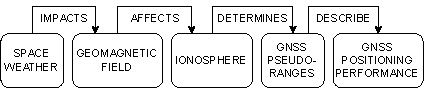
\includegraphics[width=0.89\linewidth]{SpaceWeather-TwoLines.drawio.pdf}
    \caption{The Space weather – GNSS PNT performance coupling model.}
    \label{fig:SpaceWeather}
\end{figure}

The GNSS signal encounters a certain number of charged particles from the satellite aerial to a mobile unit’s (GNSS receiver’s) aerial citestuff(schaer1999mapping, prolss2012physics). This encounter is quantified using the Total Electron Content ($TEC$) defined by Equation~1 in $electrons/m^{2}$ citestuff(spilker1996global, schaer1999mapping, davies1990ionospheric), where $h$ denotes the height above the Earth’s mean sea level in $m$, $N(h)$ represents the vertical ionospheric profile, the volume density of charged particles at height $h$, in $electrons/m^{2}$. For reasons of convenience, $TEC$ may be expressed in $TEC$ Units ($TECU$), with $1$ $TECU$ = $1016$ $electrons/m^{2}$. The $TEC$ dataset used in this study was derived from Receiver Independent Exchange Format (RINEX) $TEC$ observations using Global Positioning System (GPS) $TEC$ software by Seemala citestuff(SEEMALA202363).

\begin{equation}
	TEC = \int_{lower \quad ionospheric \quad boundary}^{upper \quad ionospheric \quad boundary}N(h)dh
	\quad\left(1\right)
\end{equation}

It should be noted that in the sense of Equation~1, $TEC$ is defined as a result, a consequence, of the ionospheric conditions, and not their descriptor citestuff(spilker1996global). The GNSS ionospheric delay may be determined by derivation from the Appleton-Hartree equation, as given in Equation~2, where $\Delta t_{iono}$ denotes the GNSS ionospheric delay in $s$, $c$ denotes the velocity of an electromagnetic wave in vacuum in $m/s$, and $f$ denotes the carrier wave frequency of the satellite signal in $Hz$ citestuff(spilker1996global, schaer1999mapping).

\begin{equation}
	\Delta t_{iono} = \frac{40.3}{c f^{2}} \int_{lower \quad ionospheric \quad boundary}^{upper \quad ionospheric \quad boundary}N(h)dh
	\quad\left(2\right)
\end{equation}

Combining Equation~1 and Equation~2, one can conclude the linear relation between $\Delta t_{iono}$ and $TEC$, as given in Equation~3 citestuff(spilker1996global).

\begin{equation}
	\Delta t_{iono} = \frac{40.3}{c f^{2}} TEC
	\quad\left(3\right)
\end{equation}

The GNSS ionospheric delay has been identified as a source of GNSS PNT degradation since the dawn of GNSS. GNSS systems offer various standard GNSS ionospheric delay estimation (correction) models to mitigate the deteriorating effects on GNSS PNT, such as the Klobuchar model citestuff(spilker1996global, klobuchar1987ionospheric). The standard ionospheric correction models are global, and insufficiently flexible to update to mitigate GNSS ionospheric delay to satisfy rising demands on GNSS PNT performance citestuff(spilker1996global, enge1994global). The development of regional and local models, such as the one presented in this paper, attempts to solve the problem of GNSS PNT sustainable performance in various ionospheric conditions. Some of the authors of this paper recently proposed the Ambient-Aware Application-Aligned ((AA)2) PNT to take into account the actual ionospheric and geomagnetic conditions near a mobile unit (a GNSS receiver) citestuff(filjar2024ambient). Direct measurements of the immediate geomagnetic and ionospheric condition variables may be supplied to a machine learning-based adapted GNSS ionospheric correction model, thus solving the single-frequency GNSS problem. Previous research has identified predictors and target variables (descriptors of geomagnetic, ionospheric, and GNSS PNT conditions) citestuff(natras2022ensemble, natras2023regional). Current space weather severity scales, such as the one provided by National Oceanic and Atmospheric Administration (NOAA), are based on global space weather and geomagnetic indices averaged over a certain period (for instance, $3$ hours for the global $K_{p}$ index). The current space weather severity scales do not directly address classifying scenarios of GNSS performance deterioration and have limited potential in deployment for a GNSS ionospheric correction model. The classification of different scenarios of GNSS ionospheric conditions with adverse effects on the GNSS PNT remained an unsolved precondition needed for the development of a machine learning-based GNSS ionospheric delay correction model to render the GNSS PNT algorithm ionospheric conditions-agnostic.

A methodology for a machine learning-based classification of ionospheric conditions based entirely on observations of geomagnetic indices is described in this study. The model is sufficiently simple to be applied on computationally capable platforms with suitable geomagnetic field sensors, such as smartphones and connected/autonomous vehicles. The research presented acquires ambient data and analyses its statistical properties. The dataset is split into training and test sets. Several candidates for the GNSS ionospheric delay model are developed based on Disturbance Storm-Time ($Dst$) data taken from the INTERMAGNET citestuff(Intermagnet2022-cj) dataset, and reformatted to match the format of $TEC$ data. The machine learning (ML) models include a Support Vector Machine (SVM) with a Polynomial Kernel, C5.0 Decision Tree (DT), Naive Bayes (NB), shallow Neural Network (NN), Partial Least Squares (PLS), Flexible Discriminant Analysis (FDA) and shallow Neural Network (NN) using Principal Component Analysis (PCA) of the input data. A tailored set of validation methods is used to assess their performance. The optimal GNSS ionospheric delay correction model is identified based on GNSS PNT-related objective criteria, and its performance is demonstrated in an independent case study.

\section{Method and data}
\label{sec:Dataset}

A Support Vector Machine (SVM) with a Polynomial Kernel, C5.0 Decision Tree (DT), Naive Bayes (NB), Neural Network (NN), Partial Least Squares (PLS), Flexible Discriminant Analysis (FDA) and shallow Neural Network (NN) using Principal Component Analysis (PCA) of the input data were tested based on their ability to classify a set of observations of the geomagnetic field in $TEC$, and other predictors, into one of the scenarios of space weather conditions based on $Dst$. Multiple $Dst$-dependent classes were predefined using theoretical knowledge. Statistical analysis of the data confirmed that distributions of other variables change for different $Dst$ ranges, supporting the validity of the classification. The study assumes that the dependent output variable, the $Dst$ class, can be predicted based on the independent variables used as input. $TEC$ data was obtained using GPS $TEC$ software by Seemala to process RINEX $TEC$ observations citestuff(SEEMALA202363). The INTERMAGNET citestuff(Intermagnet2022-cj) dataset contains $Dst$ and $a_{p}$ data from 2014 for a measuring station maintained by Geoscience Australia in Kakadu, referred to as KDU in the database, at $12.69$ degrees of south latitude and $132.47$ degrees of east longitude near Darwin, Nothern Territory, Australia. The two datasets are merged based on location, year, month, day, and time of day in hours.

\subsection{Method}
%\label{subsec:Method}

The methods were selected because they represent larger families of classification methods. SVM models are supervised maximum margin models. DT models also apply supervised learning. NB classifiers are probabilistic classifiers that can be parametric or non-parametric, but this study uses a non-parametric approach. PLS is a non-parametric linear regression model. FDA uses multiple non-parametric linear regression models to create a non-linear classification. PCA is a linear dimensionality reduction technique that extracts a predefined number of components for training an NN model. NN models imitate the brain using artificial neurons to produce outputs based on the input and the activation function. NN models require that the structure be predefined, and hyperparameters are tuned. All NN models were applied based on research by Kuhn for the \textit{R} \textit{caret} package citestuff(Kuhn2007, kuhn2008building, kuhn2013applied).

\subsubsection{Support Vector Machine}
%\label{subsubsec:SupportVectorMachine}

In machine learning, a Support Vector Machine (SVM) or Support Vector Network (SVN) model is a supervised maximum margin model with associated learning algorithms used for classification. SVM models are also effective for non-linear classification using the hyperplane kernel trick citestuff(Boser1992). Intuitively, a good separation is achieved by the hyperplane with the greatest distance to the nearest point in the training data belonging to any class citestuff(HastieRosset2009). Meyer, Leisch, and Hornik compared SVM models with other classifiers citestuff(Meyer2003). However, it is unclear whether SVM predictions perform better than other linear models, such as logistic, and linear regression. To keep the computational burden reasonable, a kernel probability density function $k(x, y)$ is chosen to fit the problem citestuff(Press2007).

\subsubsection{Decision Tree}
%\label{subsubsec:DecisionTree}

Decision Tree (DT) models are used for supervised learning in statistics and machine learning. Classification trees use a discrete target variable. DT models are popular due to their comprehensibility and simplicity citestuff(Wu2008). A tree is recursively partitioned by dividing the original set, or root node, into subsets that form descendants, or successors, using classification rules based on features citestuff(ShalevShwartz2014). C5.0, used in the \textit{caret} package in \textit{R}, has a similar approach and improves the ID3 and C4.5 algorithms.

\subsubsection{Naive Bayes}
%\label{subsubsec:NaiveBayes}

In statistics, Naive Bayes (NB) models, simple Bayes, or independent Bayes citestuff(Hand2001) classifiers are a family of linear "probabilistic classifiers" that assume that, given a target class, the features are conditionally independent. Maximum likelihood training for Naive Bayes (NB) models evaluates a closed-form expression citestuff(Russell1999) in linear time instead of using iterative approximation. However, a comprehensive comparison in 2006 showed that Naive Bayes (NB) models performed worse than boosted trees or Random Forest (RF) models citestuff(Caruana2006). An advantage of NB over other models is a smaller amount of required training data citestuff(John2013). NB models assign probabilities $p(C_{k}\mid x_{1},\ldots, x_{n})$ to $K$ classes $C_{k}$ for an input vector $x = (x_{1},\ldots, x_{n})$ with $n$ features citestuff(Murty2011), and use Bayes' theorem in Equation~4.

\begin{equation}
	p(C_{k}\mid \mathbf{x})={\frac{p(C_{k})\ p(\mathbf{x} \mid C_{k})}{p(\mathbf{x})}}
	\quad\left(4\right)
\end{equation}

\subsubsection{Neural Networks}
%\label{NeuralNetworks}

The neurons of human or animal brains provide the basis for a Neural Network (NN) or Artificial Neural Network (ANN) with connected units or nodes called artificial neurons in machine learning citestuff(brahme2014comprehensive). Shallow NN models typically contain only a few hidden layers for processing between the input layer that receives the data and the final layer that produces the output citestuff(olden2002illuminating). A network with at least two hidden layers citestuff(bishop2006pattern) is a deep NN model. Gradient-based methods such as backpropagation estimate ANN parameters citestuff(vapnik2013nature) to minimize the difference or empirical risk between the output and target labels, expressed in a loss function citestuff(goodfellow2016deep). The hyperparameters may also be modified to suit the problem citestuff(probst2019tunability) during an extensive tuning process, like the one used in this study. Principal Component Analysis (PCA) citestuff(stewart2019introduction) is a linear dimensionality reduction technique in exploratory data analysis, visualization citestuff(jolliffe2016principal), and preprocessing. The $pcaNNet$ method in the \textit{caret} package in \textit{R} uses PCA in preprocessing citestuff(Kuhn2007, kuhn2008building, kuhn2013applied).

\subsubsection{Partial Least Squares}
%\label{subsubsec:PLS}

Partial Least Squares (PLS) regression, or projection to latent structures, citestuff(abdi2010partial), is a linear regression statistical model that transforms the predicted and the observable variables to a new space. PLS methods are bilinear factor models because the $X$ and $Y$ are projected to new spaces. In Partial Least Squares Discriminant Analysis (PLS-DA), $Y$ is categorical citestuff(saebo2008lpls). Using $n$ paired observations $\left(\vec{x_{i}}, \vec{y_{i}}\right), i \in 1, \dots, n$. PLS finds the normalized direction $\vec{p_{j}}, \vec{q_{j}}$ that maximizes the covariance in the first step $j = 1$, shown in Equation~5. Many versions of PLS exist for estimating the factor and loading matrices, such as the PLS1 algorithm citestuff(GONZALEZ2023104876).

\begin{equation}
	\max_{{\vec{p}}_{j},{\vec{q}}_{j}}\operatorname{E} [\underbrace{({\vec{p}}_{j}\cdot {\vec{X}})}_{t_{j}}\underbrace{({\vec{q}}_{j}\cdot {\vec{Y}})}_{u_{j}}
	\quad\left(5\right)
\end{equation}

\subsubsection{Flexible Discriminant Analysis}
%\label{subsubsec:FDA}

Flexible Discriminant Analysis (FDA) is a general methodology that creates the discriminant surface for a multigroup non-linear classification model citestuff(mclachlan2005discriminant) based on a mixture of non-parametric linear regression models, such as Multivariate Adaptive Regression Splines (MARS) and Linear Discriminant Analysis (LDA). Many predictors can be used in conjunction in FDA citestuff(HastieTibshirani2009). FDA is complex but execution time and computational load are adequate citestuff(reynes2006choice). Feature normality and equal group covariances are assumed citestuff(wetcher2011analyzing). LDA, Normal Discriminant Analysis (NDA), or discriminant function analysis citestuff(cohen2013applied) is a generalization of Fisher's linear discriminant defined in 1936 citestuff(mclachlan2005discriminant). The results of LDA may be utilized directly for classification, as demonstrated in this experiment.

\subsection{Data description and analysis}
%\label{subsec:Data}

Dynamic space weather conditions, such as solar activity and geomagnetic storms, can affect  GNSS PNT performance and high-frequency GPS signals passing through the ionosphere, motivating work on error modeling citestuff(zolesi2014ionospheric). Geomagnetic storms cause signal deterioration by affecting Global Electric Current (GEC) variability. The ionosphere may show changes related to location, geomagnetic and solar activity, sunspots, local time, seasonality, thunderstorms citestuff(vellinov1992ionospheric), nuclear experiments, earthquakes citestuff(liu20142013), and other phenomena. This study focuses on parameters describing disturbances of the Earth's geomagnetic field, most importantly $a_{p}$-indices derived from $K_{p}$-indices, which are calculated using $K$-indices, Total Electron Content ($TEC$), standard deviation of Total Electron Content ($dTEC$), and Disturbance Storm-Time ($Dst$). Incorporating parameters such as the $K_{p}$-indices and $a_{p}$-indices, which provide global measures of geomagnetic activity, alongside local $TEC$ and $Dst$-index values, allows for a more detailed assessment of the space environment and its potential effects on GNSS signals. Values of $a_{p}$, $TEC$, $dTEC$, $Dst$ were used with the $B_x$, $B_y$, and $B_z$ components of the Earth's magnetic field to train machine-learning models.

\subsubsection{Magnetic field indices}
%\label{subsec:BxByBz}

The Earth's magnetic field has similarities to that of a bar magnet. However, plasma gushes from the solar corona and the domain of the Sun influence the interplanetary magnetic field citestuff(schwenn2001solar). The $B_{x}$, $B_{y}$, and $B_{z}$ vectors represent interplanetary magnetic field indices. $B_{x}$ and $B_{y}$ are parallel to the plane of orbits, and the third component $B_{z}$ is perpendicular. Widely available hand-held devices, such as Android smartphones citestuff(Bojinov2014), measure magnetic field indices in micro-Tesla ($\mu T$). The Android magnetometer reports accuracy through a status variable. Readings are calibrated using temperature compensation, factory (or online) soft-iron, and online hard-iron calibration.
 
\subsubsection{Geomagnetic storm indices}
%\label{subsec:K}

The geomagnetic storm $K$-index is an integer from $0$ to $9$ measuring disturbances in global geomagnetic activity. The maximum positive and negative fluctuations of the horizontal components of the Earth's magnetic field, $B_{x}$ and $B_{y}$, during $3$ hours, relative to a quiet day, are added to determine the total maximum fluctuation. Each observatory uses different threshold values to convert the maximum $nT$ (nano-Tesla) fluctuation to a $K$-index value. The thresholds for each observatory are adjusted so that the historical rate of occurrence for each $K$-index value is similar across all observatories. Observatories with a lower geomagnetic latitude use a lower fluctuation in $B_{x}$ and $B_{y}$ to achieve each $K$-index value.

\subsubsection{Planetary geomagnetic storm indices}
%\label{subsec:Kp}

The planetary geomagnetic storm $K_{p}$-index is derived from $3$-hour-based $K$-indices from $13$ magnetometer stations between $44$ and $60$ degrees of north and south latitude. Announcements and warnings of geomagnetic changes and disturbances in the Earth's magnetic field are based on the $K_{p}$-index. Hourly geomagnetic storm index data are available on the NASA Goddard SPDF web pages. The scale values of the $K_{p}$-index are determined by the change of the geomagnetic field and the geomagnetic storm effect in $nT$. The official planetary $K_{p}$-index is a weighted average of $K$-indices from multiple observatories. When $K$-index data is not available in real-time, operators such as The National Oceanic and Atmospheric Administration (NOAA) Space Weather Prediction Center (SWPC) calculate near real-time estimates of the $K_{p}$-index citestuff(Myint2022). The $K_{p}$-index is related to geomagnetic storm descriptions and warnings using the NOAA G scale. For a $K_{p}$-index value of $5$, $6$, $7$, $8$ (including $9_{-}$), and $9$, a NOAA Space Weather Scale Geomagnetic Storm Level of G1, G2, G3, G4, and G5 is assigned, respectively. For a $K_{p}$-index $<5$, the G0 designation means no warning is issued. In March 2021, $K_{p}$ was assigned a Digital Object Identifier (DOI) with a dataset citestuff(Matzka2021a) and a scientific publication citestuff(Matzka2021b) for reference.

\subsubsection{Equivalent three hourly range geomagnetic storm indices}
%\label{subsec:A}

The $A$-index represents a daily average level of magnetic activity. Because the relationship between the $K$-index and magnetometer fluctuations is not linear, the $K$-index values are not directly used for calculating average values. Each $K$-index or $K_{p}$-index is converted into the "equivalent three hourly range" $a$-index or $a_{p}$-index that uses a linear scale. An average of $8$ $a$-indices (lowercase) is used as the daily $A$-index (uppercase).  

\subsubsection{Disturbance Storm-Time}
%\label{subsubsec:Dst}

Disturbance Storm-Time ($Dst$), also known as the geomagnetic activity $Dst$-index, depicts an averaged measure of the geomagnetic storm intensity in the Earth's sub-equatorial region. The $Dst$-index is obtained by post-processing, with the final version often published months after experimental observations were collected. It clearly shows developments of various levels of geomagnetic disturbances, and consequently serves as invaluable input considering GNSS PNT performance degradation due to space weather events and disturbances. The $Dst$-index is a geomagnetic indicator of magnetic flux changes derived from measurements taken by a network of ground-based magnetometer stations near the magnetic equator, which continuously monitor $B_{x}$ and $B_{y}$, the horizontal components of Earth's magnetic field citestuff(zolesi2014ionospheric). The $Dst$-index describes ring currents forming above the sub-equatorial region and affecting the ionospheric regions in mid-latitudes. To calculate the $Dst$-index, variations in $B_{x}$ and $B_{y}$, the horizontal magnetic field, are obtained from multiple stations and averaged. The average is subtracted from a baseline value representing the quiet-time magnetic field. The resulting $Dst$ value in $nT$ measures the intensity of geomagnetic disturbances, with increasingly negative values indicating stronger geomagnetic storms. The $Dst$-indice measurements as an hourly average were evaluated and published on a web interface by the NASA Goddard SPDF, and the Geomagnetism and Space Magnetism Data Analysis Center of the Institute of Science, Kyoto University in Japan. Loewe and Prölss citestuff(loewe1997classification) classified magnetic activity $Dst$-indices into $5$ storm classes in 1997. Gonzalez et al. citestuff(gonzalez1994geomagnetic) used $3$ groups for the same data in 1994, similar to Kamide et al. in 1998 citestuff(kamide1998two), Rozhnoi et al. in 2004 citestuff(rozhnoi2004middle), and Contadakis et al. in 2012 citestuff(contadakis2012total).

\subsubsection{Training and testing dataset}
%\label{subsubsec:DataTrainTest}

The original set of observations has been split into training and testing subsets, considering the results of exploratory statistical, and outlier analysis, and sustaining proportions of data relating to classes of geomagnetic disturbances (quiet/normal geomagnetic conditions, the positive phase of a geomagnetic storm, deep negative depression of a geomagnetic storm, and the negative recovery phase of a geomagnetic storm). Classes are based on $Dst$ and differential $Dst$ time series. Out of $9799$ original samples, $208$ were marked as outliers in exploratory statistical analysis, as the $TEC$ is larger than or equal to $300$ $TECU$. $TEC$ values larger than $300$ $TECU$ usually appear due to measurement errors or errors in the $TEC$ estimation process. The remaining $9591$ samples are used for training and testing. The samples are divided into training and testing datasets as close as possible to a ratio of $80\%$ for training and $20\%$ for testing. The division was stratified so that an approximately equal ratio of classes was present in both the training and testing data, which is a feature of the \textit{createDataPartition} function from the \textit{caret} \textit{R} library that was used citestuff(Kuhn2007, kuhn2008building). Samples were split into $5$ class ranges, based on $Dst$ values derived from theoretical knowledge of different storm phases, similar to Loewe and Prölss citestuff(loewe1997classification). Table~\ref{tab:Dstranges} lists the $Dst$ class ranges used in this study, the total number of samples in each class, and the number of samples used for testing, and training.

\begin{table}[!ht]
    \centering
    \caption{$Dst$-based classification rules used in this study, the total number of samples in each class, and the number of samples used for testing, and training. The upper range limits are excluded, while the lower ones are included.}
    \label{tab:Dstranges}
    \begin{tabular}{|c|c|c|c|c|}
        \hline
        $Dst$ & Storm phase classification & Total samples & Test samples & Train samples \\ \hline
        $ \geq 15 $ & positive phase (P) & $135$ & $27$ & $108$ \\ \hline
        $[-20, 15>$ & normal (N) & $7495$ & $1499$ & $5996$ \\ \hline
        $[-55, -20>$ & recovery phase (R) & $1858$ & $371$ & $1487$ \\ \hline
        $[-85, -55>$ & through (T) & $90$ & $18$ & $72$ \\ \hline
        $ < -85$ & extreme (E) & $13$ & $2$ & $11$ \\ \hline
        Any & Any & $95$ & $2$ & $11$ \\ \hline
    \end{tabular}
\end{table}

It is evident from Table~\ref{tab:Dstranges} that the normal (N), and recovery (R) classes are more common than those with very high or low $Dst$ values, impacting model performance.

\subsubsection{Data preprocessing}
%\label{subsubsec:Preprocessing}

Data preprocessing can increase classification accuracy citestuff(Fan2008). There are many ways to standardize data, such as minimum-maximum, normalization by decimal scaling, and Z-score citestuff(Mohamad2013). Subtracting the mean and dividing by the variance for each feature are commonly used for SVM models citestuff(Fennell2019) and other models tested in this study, so this approach was chosen. The values \textit{scale} and \textit{center} were used in this study in the \textit{preProcess} parameter for the \textit{train} function from the \textit{R} \textit{caret} package. The option \textit{center} subtracts the mean of each feature while \textit{scale} divides by the standard deviation.

\subsubsection{Distribution analysis for predictors}
%\label{subsubsec:Distribution}

Table~\ref{tab:minmax} provides the minimum, $1^{st}$ quartile, median, arithmetic mean, $3^{rd}$ quartile, and maximum values for all variables when the $TEC$ is less than $300$ $TECU$, suggesting that variables are not normally distributed.

\begin{table}[!ht]
    \centering
    \caption{The minimum, $1^{st}$ quartile, median, arithmetic mean, $3^{rd}$ quartile, and maximum values for all variables when the $TEC$ is less than $300$ $TECU$.}
    \label{tab:minmax}
        \begin{tabular}{|c|c|c|c|c|c|c|c|}
                \hline
                  & $TEC$ & $dTEC$ & $B_{x}$ & $B_{y}$ & $B_{z}$ & $Dst$ & $a_{p}$ \\ \hline
                Min. & $1.76$ & $0.02$ & $35275.0$ & $1913.0$ & $-29649.0$ & $-119.0$ & $0.0$ \\ \hline
                $1^{st}$ Qu. & $8.43$ & $1.12$ & $35402.0$ & $1990.0$ & $-29623.0$ & $-18.0$ & $4.0$ \\ \hline
                Median & $22.83$ & $2.47$ & $35410.0$ & $2004.0$ & $-29620.0$ & $-5.0$ & $6.0$ \\ \hline
                Mean & $24.62$ & $6.208$ & $35413.0$ & $2003.0$ & $-29617.0$ & $-9.678$ & $7.539$ \\ \hline
                $3^{rd}$ Qu. & $34.23$ & $5.54$ & $35423.0$ & $2018.0$ & $-29614.0$ & $-1.0$ & $7.0$ \\ \hline
                Max. & $288.0$ & $997.0$ & $35524.0$ & $2089.0$ & $-29571.0$ & $46.0$ & $94.0$ \\ \hline
        \end{tabular}
\end{table}

The Kolmogorov-Smirnov and Shapiro-Wilk normality tests, using \textit{R} functions \textit{ks.test} and \textit{shapiro.test}, did not yield a $p$-value larger than the selected $\alpha$-value of $0.05$ for any variable, further strengthening the claim based on Table~\ref{tab:minmax} that variables do not follow a normal (Gaussian) distribution.
  
\subsubsection{Correlation analysis for predictors}
%\label{subsubsec:Correlation}

Observations of statistical variables were assessed for their mutual association/correlation to identify the classification model structure, potential predictors, and targets. Figure~\ref{fig:correlation} contains a heat map of the correlation between all variables used in the study.

\begin{figure}[!ht]
 \centering
 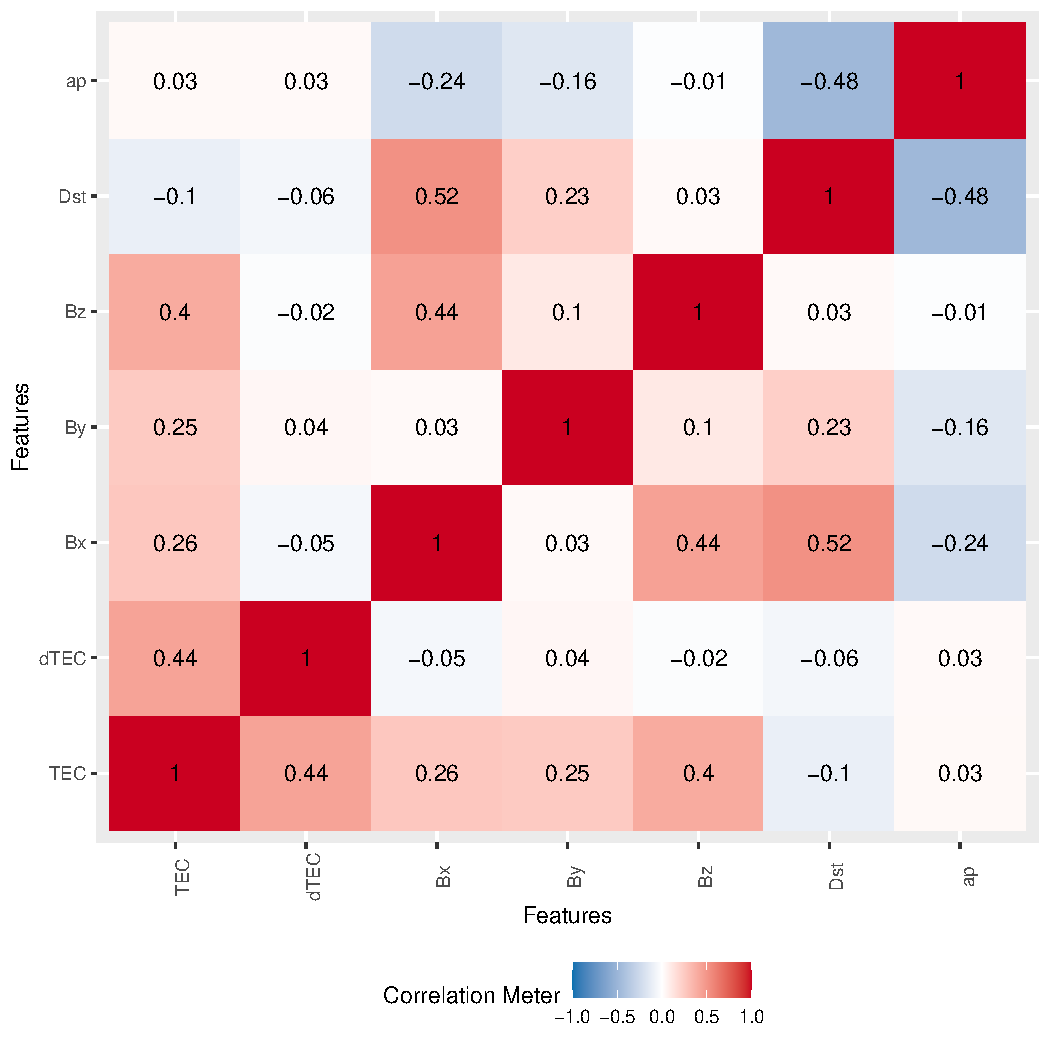
\includegraphics[width=0.7\linewidth]{iono3correlation.pdf}
    \caption{A heat map of the correlation between all variables used in this study, when the $TEC$ is less than $300$ $TECU$. Red represents a high positive correlation, blue represents a high negative correlation, and white represents a low correlation. Variables are fully correlated with themselves, so values on the secondary diagonal equal $1$. The matrix is symmetrical concerning the secondary diagonal because the same combination of correlated variables is achieved when swapping the row and column indices.}
    \label{fig:correlation}
\end{figure}

The $B_{x}$ and $Dst$ variables exhibit the largest correlation coefficient in Figure~\ref{fig:correlation}, equaling $0.52$. The association between the two variables seems logical since the $Dst$ index is defined as a result of geomagnetic field conditions described by geomagnetic field components. The second largest correlation coefficient depicts a significant correlation between $a_{p}$ and $Dst$ and equals $-0.48$, thus confirming that the $a_{p}$ variable can be used as a predictor, with the $Dst$ variable as a target, and an opposite trend.

The box plots of all variables for different ranges of $Dst$ values in Figure~\ref{fig:iono3boxplot} are used to support the correlations shown in Figure~\ref{fig:correlation} by exhibiting the trend of each variable.

\begin{figure}[!ht]
    \centering
    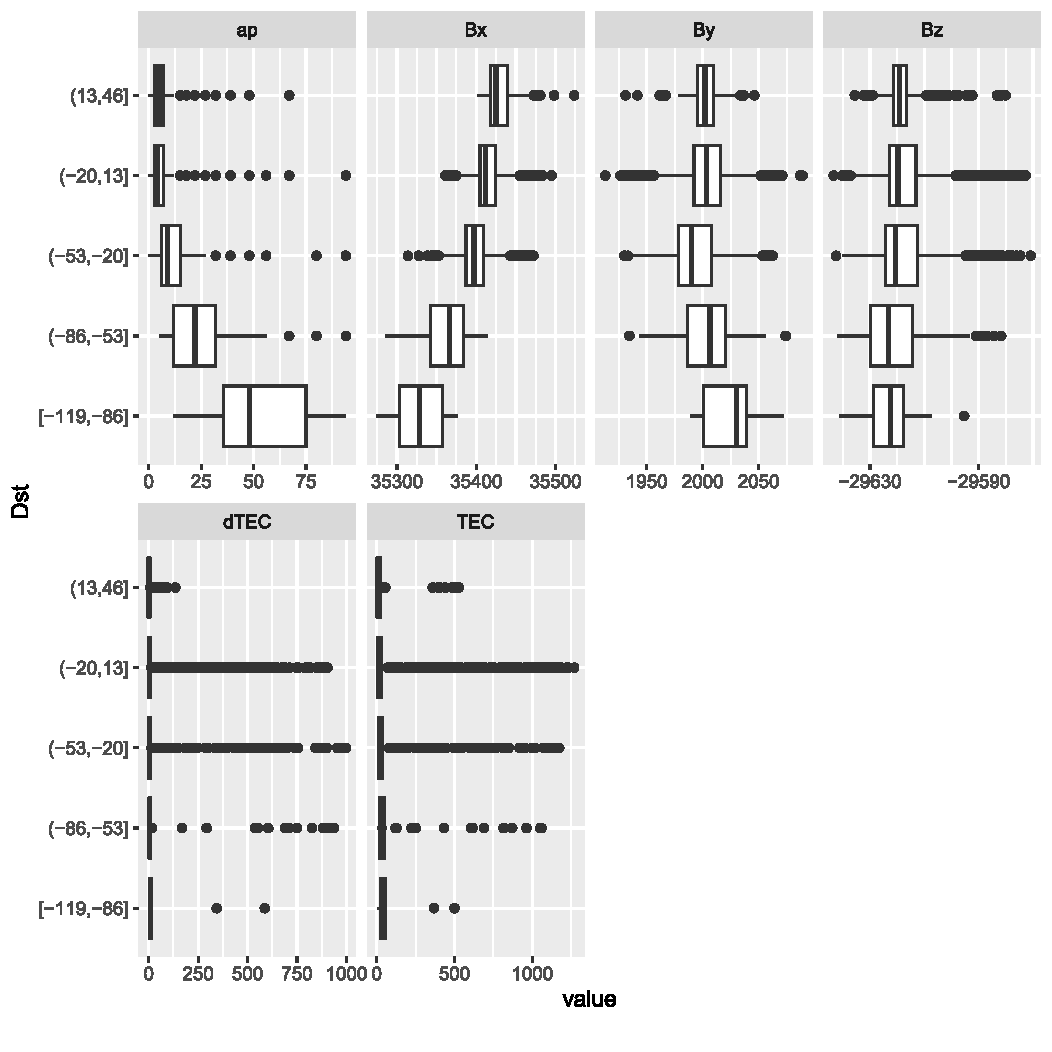
\includegraphics[width=\linewidth]{iono3boxplot_fix.pdf}
    \caption{Box plots of all variables, when the $TEC$ is less than $300$ $TECU$, for different ranges of $Dst$ values defining the class label used in this study.}
    \label{fig:iono3boxplot}
\end{figure}

Figure~\ref{fig:iono3boxplot} shows the minimum, maximum, and arithmetic mean of $a_{p}$ decreasing for larger $Dst$ values. The opposite is true for $B_{x}$, as indicated by a high correlation in Figure~\ref{fig:correlation}. $B_{y}$ exhibits a reverse trend compared to $B_{x}$, but it is less prominent. $B_{z}$ is the most stable among geomagnetic indices, with the smallest changes related to $Dst$.

\subsection{Confusion Matrix}
%\label{subsec:Metrics}

The metrics and terminology defined in the \textit{R} function \textit{confusionMatrix} in the \textit{caret} library citestuff(Kuhn2007, kuhn2008building) were used to evaluate classifier performance. The default approach to a confusion matrix uses only two groups (Yes and No, positive and negative). For multiple classes, results are calculated by a "one versus all" approach, viewing each class as positive and all others as negative.

\subsubsection{McNemar-Bowker test}
%\label{subsubsec:McNemar}

McNemar’s test for correlated proportions used on paired categorical data is based on the chi-squared distribution and was originally designed for methods that differentiate between two classes. The null hypothesis of marginal homogeneity states that marginal probabilities for each outcome are equal, which is more indicative of model difference than directly comparing the sensitivity and specificity of two candidate models.

However, for $k$ groups, the classification can be annotated
in a $k \times k$ contingency table with the number of samples classified using the first method in separate rows by class, divided into columns depending on the class assigned by the opposing method. The McNemar-Bowker test is applied to this table, formulated by Fagerland et al. citestuff(fagerland2017statistical), and Chow et al. citestuff(chow2018sample).

If any element in the matrix is smaller than $6$, as shown using class sizes in Table~\ref{tab:Dstranges}, the distribution is not well-approximated by the chi-squared distribution. Edwards citestuff(edwards1948note) developed an approximation of the binomial exact $p$-value for continuity-correction, given in Equation~6 for two groups. In Equation~6, $b$ is the number of samples classified in the first group by the first test, and the second group by the second test, while $c$ is the number of samples for which the opposite is true.
 
\begin{equation}
	\chi^{2}=\frac{(|b-c|-1)^{2}}{b+c}
	\quad\left(6\right)
\end{equation}

\section{Research results}
\label{sec:Results}

Candidate models were assessed to determine the optimal method and set of predictors to be used in the final model for application in real settings. The accuracy and the execution time in seconds ($s$) utilizing the \textit{R} \textit{system.time} function for all candidate models are displayed in Table~\ref{tab:acc:time}. Research results are presented with the following initial set of six predictors: Total Electron Content ($TEC$), standard deviation of Total Electron Content ($dTEC$), $B_{x}$, $B_{y}$, $B_{z}$, and $a_{p}$. $Dst$ was not used as a predictor since the initial classification is derived from $Dst$ values. Candidate models have also been developed using: (1.): all predictors except $TEC$, and $dTEC$ ($B_{x}$, $B_{y}$, $B_{z}$, and $a_{p}$), (2.): Geomagnetic indices ($B_{x}$, $B_{y}$, and $B_{z}$), (3.): $B_{x}$, $B_{y}$, and $a_{p}$, (4.): $B_{x}$, $B_{z}$, and $a_{p}$, and (5.): $B_{y}$, $B_{z}$, and $a_{p}$. The reasoning behind this approach was the assumption that reducing the set of predictors would reduce model complexity and computation time. Additionally, it is theoretically established that geomagnetic indices $B_{x}$, $B_{y}$, and $B_{z}$ affect $Dst$, and in turn $TEC$. This is why geomagnetic indices ($B_{x}$, $B_{y}$, and $B_{z}$), and $a_{p}$ were used as predictors in the final model. The highest accuracy in Table~\ref{tab:acc:time} was achieved using $B_{x}$, $B_{y}$, $B_{z}$, and $a_{p}$ as predictors, supporting the hypothesis that $TEC$, and $dTEC$ should be removed from the set of predictors. The Naive Bayes (NB) method yielded the model with the highest accuracy, leading to the decision that it should be used in the final model.

\begin{table}[!ht]
    \centering
    \caption{The accuracy (top) and the execution time in seconds ($s$) (bottom) for each candidate model developed using different methods and sets of predictors.}
	\label{tab:acc:time}
	\begin{tabular}{|c|c|c|c|c|c|c|}
		\hline
        Candidate & \multicolumn{6}{|c|}{Accuracy} \\ \cline{2-7}
        model & \multicolumn{6}{|c|}{Predictors} \\ \hline
		Method & All & $B_{x}$, $B_{y}$, $B_{z}$, $a_{p}$ & $B_{x}$, $B_{y}$, $B_{z}$ & $B_{x}$ $B_{y}$ $a_{p}$ & $B_{x}$ $B_{z}$ $a_{p}$ & $B_{y}$ $B_{z}$ $a_{p}$ \\ \hline
		SVM Poly & $0.7454$ & $0.7903$ & $0.7887$ & $0.7934$ & $0.7903$ & $0.7814$ \\ \hline
		C5.0 DT & $0.8529$ & $0.8581$ & $0.8404$ & $0.8508$ & $0.8367$ & $0.8211$ \\ \hline
		NB & $0.9943$ & $1$ & $1$ & $1$ & $1$ & $0.9995$ \\ \hline
		NN & $1$ & $1$ & $1$ & $1$ & $1$ & $1$ \\ \hline
		PLS & $0.8258$ & $0.8232$ & $0.8174$ & $0.8153$ & $0.8143$ & $0.8007$ \\ \hline
		FDA & $0.8472$ & $0.8472$ & $0.8252$ & $0.8419$ & $0.8258$ & $0.7997$ \\ \hline
		PCA NN & $0.8492$ & $0.8492$ & $0.8399$ & $0.8456$ & $0.8367$ & $0.8185$ \\ \hline
        Candidate & \multicolumn{6}{|c|}{Execution time in seconds ($s$)} \\ \cline{2-7}
        model & \multicolumn{6}{|c|}{Predictors} \\ \hline
		Method & All & $B_{x}$, $B_{y}$, $B_{z}$, $a_{p}$ & $B_{x}$, $B_{y}$, $B_{z}$ & $B_{x}$ $B_{y}$ $a_{p}$ & $B_{x}$ $B_{z}$ $a_{p}$ & $B_{y}$ $B_{z}$ $a_{p}$ \\ \hline
		SVM Poly & $337.38$ & $391.42$ & $565.11$ & $727.45$ & $649.28$ & $856.54$ \\ \hline
		C5.0 DT & $681.36$ & $470.88$ & $350.02$ & $360.72$ & $333.90$ & $388.50$ \\ \hline
		NB & $207.13$ & $170.22$ & $145.93$ & $149.69$ & $151.67$ & $155.84$ \\ \hline
		NN & $630.47$ & $617.97$ & $590.97$ & $616.92$ & $632.41$ & $651.09$ \\ \hline
		PLS & $61.29$ & $52.75$ & $36.47$ & $51.37$ & $41.37$ & $59.63$ \\ \hline
		FDA & $92.49$ & $135.62$ & $141.52$ & $159.61$ & $167.59$ & $187.72$ \\ \hline
		PCA NN & $420.25$ & $460.76$ & $449.86$ & $475.48$ & $491.82$ & $524.88$ \\ \hline
	\end{tabular}
\end{table}

The experiment was run on \textit{Windows} 11 using \textit{R Studio} version 2024.04.2+764 and \textit{R} version 4.4.1, the AMD Radeon RX 6600 Graphics Processing Unit (GPU), $16$ GB of Random Access Memory (RAM), and the AMD Ryzen 5 PRO 4650G Central Processing Unit (CPU) with $6$ cores. Execution time is significant because built-in systems for mobile devices using GNSS PNT have low computational capabilities. The candidate models using the Partial Least Squares (PLS) method in Table~\ref{tab:acc:time} have the lowest execution time.

The performance assessment of candidate models revealed the success of several methods, such as the Neural Network (NN) and Naive Bayes (NB) classifiers. Accuracy results in Table~\ref{tab:acc:time} may lead to an incorrect conclusion as the dataset is unbalanced, as shown in Table~\ref{tab:Dstranges}. Further assessment is needed to determine if a candidate model differs significantly from others. The results of
McNemar’s test are presented only for candidate models using either the Naive Bayes (NB) method or $B_{x}$, $B_{y}$, $B_{z}$, and $a_{p}$ as predictors variables, as this combination presented as the most accurate among tested candidate models and has a lower computational load than competing models.

\subsection{Results of McNemar's test}
%\label{subsec:ResultsMcNemar}

McNemar’s test can help assess if a candidate model performs significantly worse or better than others. Figure~\ref{fig:pvalueplot} contains $p$-values of McNemar's test when comparing candidate models using the Naive Bayes (NB) method and various predictor variable sets, or $B_{x}$, $B_{y}$, $B_{z}$, and $a_{p}$ as predictor variables combined with various classification methods. A higher $p$-value indicates that the marginal probabilities for classification outcomes are unequal for a pair of candidate models, and the null hypothesis can be rejected. A lower $p$-value indicates that the marginal probabilities for classification outcomes are the same for a pair of candidate models, and the null hypothesis cannot be rejected.

\begin{figure}[!ht]
 \centering
    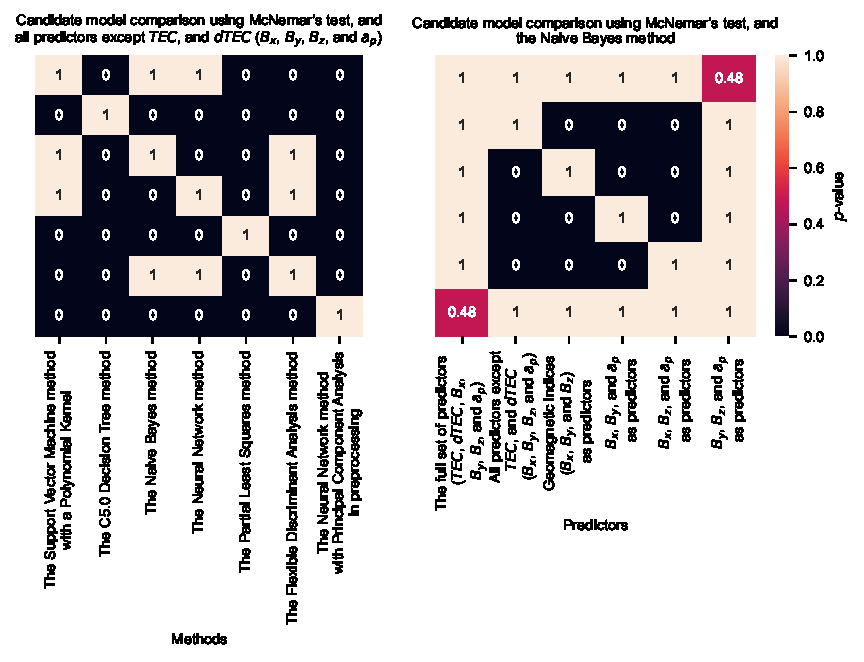
\includegraphics[width=\linewidth]{pvalueplot_total_horizontal.pdf}
    \caption{Candidate model comparison using $p$-values of McNemar's test, and $B_{x}$, $B_{y}$, $B_{z}$, and $a_{p}$ as predictor variables (excluding Total Electron Content ($TEC$), and standard deviation of Total Electron Content ($dTEC$)) combined with various classification methods (left), or the Naive Bayes (NB) method combined with various predictor variable sets (right). Black represents a low $p$-value near $0$, white represents a high $p$-value near $1$, and red represents a $p$-value near $0.5$ between the two extremes. Each candidate model is equal to itself, so values on the primary diagonal equal $1$. The matrix is symmetrical concerning the primary diagonal because the same result is achieved when swapping the order of the first and second compared candidate models.}
    \label{fig:pvalueplot}
\end{figure}

The marginal probabilities for each outcome are different when comparing the candidate model using the NB method, and $B_{x}$, $B_{y}$, $B_{z}$, and $a_{p}$ predictor variables, to the models using the same method, and the full set of predictors (Total Electron Content ($TEC$), standard deviation of Total Electron Content ($dTEC$), $B_{x}$, $B_{y}$, $B_{z}$, and $a_{p}$), or $B_{y}$, $B_{z}$, and $a_{p}$ as predictors.

This was concluded by rejecting the null hypothesis using $p$-values of McNemar's test that equal $1$, as given in Figure~\ref{fig:pvalueplot}. The $p$-values support the conclusion based on accuracy values, which are highest when using $B_{x}$, $B_{y}$, $B_{z}$, and $a_{p}$. This adds validity to removing $TEC$, and $dTEC$ from the set of predictors.

The marginal probabilities for each outcome are different when comparing the candidate model using $B_{x}$, $B_{y}$, $B_{z}$, and $a_{p}$ as predictor variables, and the NB method, to the models using the same set of predictors, and the SVM method with a Polynomial Kernel, or the FDA method. The $p$-values of McNemar's test that equal $1$, as shown in Figure~\ref{fig:pvalueplot}, add validity to accuracy comparison results, which indicate a lower accuracy when using a method other than NB and predictors other than $B_{x}$, $B_{y}$, $B_{z}$, and $a_{p}$.

\section{Discussion}
\label{sec:Discussion}

The Support Vector Machine (SVM) method with a Polynomial Kernel, C5.0 Decision Tree (DT), Neural Network (NN), and NN method with Principal Component Analysis (PCA) applied in preprocessing have the highest execution time, above $300$ $s$, so they were excluded from further analysis and application in the final model.

The Neural Network (NN) method has a high execution time for any set of predictors due to its complexity and extensive training, evident from the data in Table~\ref{tab:acc:time}. However, it achieved a $100\%$ accuracy, also shown in Table~\ref{tab:acc:time}. The Naive Bayes (NB) method has the same accuracy when using $B_{x}$, $B_{y}$, $B_{z}$, and $a_{p}$ as predictors, and the training time for the NN model is more than twice as long, so the NB method is preferred as the approach in the final model.

An analysis in 2004 showed reasonable theoretical reasons for the seemingly incredible performance of NB classifiers citestuff(Zhang2004). The expression used for the NB method is a linear time algorithm if time complexity is expressed as a function of the size of the input and observing asymptotic behavior, explaining the reduced execution time citestuff(Russell1999). Despite their simplicity, NB classifier models have performed well in real-world situations citestuff(Metsis2006), even with a relative lack of data compared to other approaches citestuff(John2013, Mccallum2001).

All candidate models developed using methods other than NN and NB fail to achieve accuracy over $90\%$. This indicates that they are less suitable for this particular application. The SVM method with a Polynomial Kernel is consistently the worst-performing for any set of predictors, never achieving an accuracy over $80\%$. All models achieved an accuracy over $70\%$, suggesting they could indicate Global Navigation Satellite System (GNSS) Positioning, Navigation, and Timing (PNT) performance.

\section{Conclusion}
\label{sec:Conclusion}

The presented study aims to classify ambient conditions of space weather events for sub-equatorial regions. Global Navigation Satellite System (GNSS) Positioning, Navigation, and Timing (PNT) performance is significantly affected by such events. It would be beneficial to warn users of a geomagnetic/ionospheric storm.

Classification models using machine learning were applied to descriptions of the geomagnetic field expressed in Total Electron Content ($TEC$), standard deviation of Total Electron Content ($dTEC$), $B_{x}$, $B_{y}$, $B_{z}$ (geomagnetic field indices), and $a_{p}$. It was assumed observations contained independent variables to generate the dependent variable representing the Disturbance Storm-Time ($Dst$) class. 

Statistical analysis confirmed that other variables change distribution based on $Dst$, not $TEC$. Continuous $Dst$ values in different ranges were converted into discrete classes based on statistics, previous theories, and research. 

An Support Vector Machine (SVM) with a Polynomial Kernel, C5.0 Decision Tree (DT), Naive Bayes (NB), Neural Network (NN), Partial Least Squares (PLS), Flexible Discriminant Analysis (FDA), and Principal Component Analysis (PCA) NN model created a $Dst$-based classification from multiple combinations of input variables.

The NB method using $B_{x}$, $B_{y}$, $B_{z}$, and $a_{p}$ as predictors achieved perfect accuracy on the test set. The total execution time is at least two times shorter than for the NN method, making it more suitable for compact, low-performance, and low-cost portable devices such as smartphones. The exclusion of $TEC$ and $dTEC$ is supported by theory since they contain redundant information already presented by $B_{x}$, $B_{y}$, and $B_{z}$ which impact $Dst$, and in turn  $TEC$.

\clearpage

\section{Acronyms}
\label{sec:Acronyms}

\textit{(AA)2} Ambient-Aware Application-Aligned


\\[2\baselineskip]

\textit{ANN} Artificial Neural Network


\\[2\baselineskip]

\textit{BA} Balanced Accuracy


\\[2\baselineskip]

\textit{CCA} Canonical Correlation Analysis

\textit{CI} Confidence Interval

\textit{CNN} Convolutional Neural Network

\textit{CPU} Central Processing Unit


\\[2\baselineskip]

\textit{DBSCAN} Density-Based Spatial Clustering

\textit{DOI} Digital Object Identifier

\textit{DP} Detection Prevalence

\textit{DR} Detection Rate

\textit{DT} Decision Tree

\textit{Dst} Disturbance Storm-Time


\\[2\baselineskip]

\textit{EOF} Empirical Orthogonal Functions

\textit{EPB} Equatorial Plasma Bubbles

\textit{EUV} Extreme ultraviolet

\textit{EVD} Eigenvalue Decomposition


\\[2\baselineskip]

\textit{FDA} Flexible Discriminant Analysis

\textit{FN} False Negative

\textit{FP} False Positive


\\[2\baselineskip]

\textit{GEC} Global Electric Current

\textit{GFZ} German Research Centre for Geosciences

\textit{GNSS} Global Navigation Satellite System

\textit{GPS} Global Positioning System

\textit{GPU} Graphics Processing Unit


\\[2\baselineskip]

\textit{ION} The Institute of Navigation


\\[2\baselineskip]

\textit{KLT} Karhunen–Loève Theorem


\\[2\baselineskip]

\textit{LDA} Linear Discriminant Analysis


\\[2\baselineskip]

\textit{MANOVA} Multivariate Analysis Of Variance

\textit{MARS} Multivariate Adaptive Regression Splines

\textit{ML} machine learning


\\[2\baselineskip]

\textit{NAS} Neural Architecture Search

\textit{NASA} National Aeronautics and Space Administration

\textit{NB} Naive Bayes

\textit{NDA} Normal Discriminant Analysis

\textit{NIR} No Information Rate

\textit{NN} Neural Network

\textit{NOAA} National Oceanic and Atmospheric Administration

\textit{NPV} Negative Predictive Value

\textit{NRCAN} Natural Resources Canada


\\[2\baselineskip]

\textit{PCA} Principal Component Analysis

\textit{PLS} Partial Least Squares

\textit{PLS-DA} Partial Least Squares Discriminant Analysis

\textit{PNT} Positioning, Navigation, and Timing

\textit{POD} Proper Orthogonal Decomposition

\textit{PPV} Positive Predictive Value


\\[2\baselineskip]

\textit{RAM} Random Access Memory

\textit{RF} Random Forest

\textit{RIN} The Royal Institute of Navigation

\textit{RINEX} Receiver Independent Exchange Format


\\[2\baselineskip]

\textit{SAR} Synthetic Aperture Radar

\textit{SPDF} Space Physics Data Facility

\textit{SVD} Singular Value Decomposition

\textit{SVM} Support Vector Machine

\textit{SVN} Support Vector Network

\textit{SWPC} Space Weather Prediction Center


\\[2\baselineskip]

\textit{TDIDT} Top-Down Induction of Decision Trees

\textit{TEC} Total Electron Content

\textit{TID} Traveling Ionospheric Disturbance

\textit{TN} True Negative

\textit{TNR} True Negative Rate

\textit{TP} True Positive

\textit{TPR} True Positive Rate


\\[2\baselineskip]

\textit{URSI} Union Radio-Scientifique Internationale


\\[2\baselineskip]

\textit{dTEC} standard deviation of Total Electron Content



\section{Declarations}
%\label{sec:Declarations}

\subsection{Availability of data and materials}
%\label{subsec:Availability}

The datasets used during the current study are available from the corresponding author upon reasonable request.

\subsection{Competing interests}
%\label{subsec:Competing}

The authors declare no conflict of interest.

\subsection{Funding}
%\label{subsec:Funding}

The authors have no funding sources to declare.

\subsection{Authors' contributions}
%\label{subsec:Contributions}

L\v{Z} contributed to conceptualization, methodology, software, validation, formal analysis, investigation, data curation, original draft writing, text review and editing, and visualization. DK contributed to conceptualization, methodology, investigation, original draft writing, and text review and editing. TI contributed to validation, formal analysis, investigation, text review and editing, supervision, and project administration. RF contributed to conceptualization, methodology, investigation, resources, original draft writing, text review and editing, and supervision. All authors read and approved the final manuscript.

\subsection{Acknowledgements}
%\label{subsec:Acknowledgements}

Not applicable

\subsection{Authors' information}
%\label{subsec:Information}

L\v{Z} is a doctoral student at the Faculty of Engineering, University of Rijeka, currently employed as an assistant at the Department of Computer Science. Her research interests include applied machine learning in biology, chemistry, medicine, and transportation. Maritime transportation is also the subject of her doctoral research.

DK is a doctoral student at the Faculty of Engineering, University of Rijeka, currently employed as an assistant at the Department of Computer Science. His research interests include applied machine learning in object recognition and image segmentation. Image classification and labeling are also the subject of his doctoral research.

TI earned his MSc and PhD in telecommunication engineering from the University of Ruse “Angel Kanchev,” Ruse, Bulgaria, in 1999 and 2007, respectively. He is a full professor at the Department of Telecommunication, University of Ruse “Angel Kanchev.” His research interests include mobile communications networks, signal processing, wireless technologies, and satellite navigation. Professor Iliev is a Member of IEEE.

RF is an external Professor of Electronics Engineering with the Department for Computer Science, Faculty of Engineering, and Center for Artificial Intelligence and Cybersecurity, both at the University of Rijeka, Croatia, and Head of the Laboratory for Spatial Intelligence at Hrvatsko Zagorje Krapina University of Applied Science, Krapina, Croatia. He holds a BSc, MSc, and PhD in electrical engineering, obtained in 1987, 1994, and 2007, respectively, from the Faculty of Electrical Engineering and Computing, University of Zagreb, Croatia. His professional interests include Ambient-Aware Application-Aligned ((AA)2) Global Navigation Satellite System (GNSS) Positioning, Navigation, and Timing (PNT), spatial uncertainty quantification, spatial statistical learning, predictive modeling, statistical signal processing, trajectory analysis and prediction, and occupancy modeling. Professor Filjar is a Fellow of The Royal Institute of Navigation (RIN) (London, United Kingdom), a Member of The Institute of Navigation (ION) (Manassas, Virginia), a Senior Member of Union Radio-Scientifique Internationale (URSI) (Ghent, Belgium) and a Member of The Society for Industrial and Applied Mathematics  (Philadelphia, Philadelphia).

%%===========================================================================================%%
%% If you are submitting to one of the Nature Portfolio journals, using the eJP submission   %%
%% system, please include the references within the manuscript file itself. You may do this  %%
%% by copying the reference list from your .bbl file, paste it into the main manuscript .tex %%
%% file, and delete the associated \verb+\bibliography+ commands.                            %%
%%===========================================================================================%%

\section{Bibliography}
%\label{sec:Bibliography}
[1] J. J. Spilker Jr, P. Axelrad, B. W. Parkinson, and P. Enge, Global positioning system: theory and applications, volume I. Reston, Virginia: American Institute of Aeronautics, 1996.

[2] S. Schaer, Mapping and predicting the Earth’s ionosphere using the Global Positioning System, vol. 59. Zürich: Institut für Geodäsie und Photogrammetrie, Eidg. Technische Hochschule, 1999.

[3] M. Durmaz and M. O. Karslioglu, “Regional vertical total electron content (VTEC) modeling together with satellite and receiver differential code biases (DCBs) using semi-parametric multivariate adaptive regression B-splines (SP-BMARS),” Journal of Geodesy, vol. 89, pp. 347–360, 2015, doi: 10.1007/s00190-014-0779-8.

[4] R. Jin, S. Jin, and G. Feng, “M_DCB: Matlab code for estimating GNSS satellite and receiver differential code biases,” GPS solutions, vol. 16, no. 4, pp. 541–548, 2012, doi: 10.1007/s10291-012-0279-3.

[5] K. Davies, Ionospheric Radio. Futures Place, Stevenage: Institution of Engineering & Technology, 1990. [Online] . Available: https://books.google.hr/books?id=qdWUKSj5PCcC

[6] J. Y. Liu et al., “Seismoionospheric GPS total electron content anomalies observed before the 12 May 2008 Mw7. 9 Wenchuan earthquake,” Journal of Geophysical Research: Space Physics, vol. 114, no. A4, 2009, doi: 10.1029/2008JA013698.

[7] G. Prölss, Physics of the Earth’s space environment: an introduction. Berlin/Heidelberg, Germany: Springer Science & Business Media, 2012.

[8] A. Oxley, Uncertainties in GPS Positioning: A mathematical discourse. Cambridge, Massachusetts: Academic Press, 2017.

[9] G. K. Seemala, “Chapter 4 - Estimation of ionospheric total electron content (TEC) from GNSS observations,” in Atmospheric Remote Sensing, A. K. Singh and S. Tiwari, Eds. Amsterdam, Netherlands: Elsevier, 2023, pp. 63–84. doi: 10.1016/B978-0-323-99262-6.00022-5.

[10] J. A. Klobuchar, “Ionospheric time-delay algorithm for single-frequency GPS users,” IEEE Transactions on aerospace and electronic systems, pp. 325–331, 1987, doi: 10.1109/TAES.1987.310829.

[11] P. K. Enge, “The global positioning system: Signals, measurements, and performance,” International Journal of Wireless Information Networks, vol. 1, pp. 83–105, 1994, doi: 10.1007/BF02106512.

[12] R. Filjar, I. Hedji, J. Prpić-Oršić, and T. Iliev, “An Ambient Adaptive Global Navigation Satellite System Total Electron Content Predictive Model for Short-Term Rapid Geomagnetic Storm Events,” Remote Sensing, vol. 16, no. 16, p. 3051, 2024, doi: 10.3390/rs16163051.

[13] R. Natras, B. Soja, and M. Schmidt, “Ensemble machine learning of random forest, AdaBoost and XGBoost for vertical total electron content forecasting,” Remote Sensing, vol. 14, no. 15, p. 3547, 2022, doi: 10.3390/rs14153547.

[14] R. Natras et al., “Regional ionosphere delay models based on CORS data and machine learning,” NAVIGATION: Journal of the Institute of Navigation, vol. 70, no. 3, 2023, doi: 10.33012/navi.577.

[15] INTERMAGNET and others, “Intermagnet reference data set (IRDS) 2019 – definitive magnetic observatory data,” GFZ Data Services, 2022, doi: 10.5880/INTERMAGNET.1991.2019.

[16] M. Kuhn, “caret: Classification and Regression Training,” CRAN: Contributed Packages, Oct. 2007, doi: 10.32614/cran.package.caret.

[17] M. Kuhn, “Building predictive models in R using the caret package,” Journal of statistical software, vol. 28, pp. 1–26, 2008, doi: 10.18637/jss.v028.i05.

[18] M. Kuhn, Applied predictive modeling. Berlin/Heidelberg, Germany: Springer, 2013.

[19] B. E. Boser, I. M. Guyon, and V. N. Vapnik, “A training algorithm for optimal margin classifiers,” in Proceedings of the fifth annual workshop on Computational learning theory, Jul. 1992, pp. 144–152. doi: 10.1145/130385.130401.

[20] T. Hastie, S. Rosset, J. Zhu, and H. Zou, “Multi-class AdaBoost,” Stat. Interface, vol. 2, no. 3, pp. 349–360, 2009, doi: 10.4310/SII.2009.v2.n3.a8.

[21] D. Meyer, F. Leisch, and K. Hornik, “The support vector machine under test,” Neurocomputing, vol. 55, no. 1–2, pp. 169–186, Sep. 2003, doi: 10.1016/S0925-2312(03)00431-4.

[22] W. H. Press, S. A. Teukolsky, W. T. Vetterling, and B. P. Flannery, Numerical recipes 3rd edition, Third. Cambridge, England: Cambridge University Press, 2007.

[23] X. Wu et al., “Top 10 algorithms in data mining,” Knowl. Inf. Syst., vol. 14, no. 1, pp. 1–37, Jan. 2008, doi: 10.1007/s10115-007-0114-2.

[24] S. Shalev-Shwartz and S. Ben-David, “Decision Trees,” in Understanding Machine Learning: From Theory to Algorithms, Cambridge, England: Cambridge University Press, 2014, pp. 212–218. doi: 10.1017/CBO9781107298019.019.

[25] D. J. Hand and K. Yu, “Idiot’s Bayes: Not So Stupid after All?,” Int. Stat. Rev., vol. 69, no. 3, p. 385, Dec. 2001, doi: 10.1111/j.1751-5823.2001.tb00465.x.

[26] S. J. Russell and P. Norvig, Artificial intelligence: a modern approach. London, England: Pearson, 2016.

[27] R. Caruana and A. Niculescu-Mizil, “An Empirical Comparison of Supervised Learning Algorithms,” Proceedings of the 23rd international conference on Machine learning - ICML ’06, vol. 2006, pp. 161–168, Jun. 2006, doi: 10.1145/1143844.1143865.

[28] G. H. John and P. Langley, “Estimating Continuous Distributions in Bayesian Classifiers,” arXiv preprint arXiv:1302.4964, 2013, doi: 10.48550/arXiv.1302.4964.

[29] M. N. Murty and V. S. Devi, Pattern recognition: An algorithmic approach. Berlin/Heidelberg, Germany: Springer Science & Business Media, 2011.

[30] A. Brahme, Comprehensive biomedical physics. 8-11 Southampton Street, London: Newnes, 2014.

[31] J. D. Olden and D. A. Jackson, “Illuminating the ‘black box’: a randomization approach for understanding variable contributions in artificial neural networks,” Ecological modelling, vol. 154, no. 1–2, pp. 135–150, 2002, doi: 10.1016/S0304-3800(02)00064-9.

[32] C. Bishop, Pattern Recognition and Machine Learning. Berlin/Heidelberg, Germany: Springer, 2006.

[33] V. Vapnik, The nature of statistical learning theory. Berlin/Heidelberg, Germany: Springer science & business media, 2013.

[34] I. Goodfellow, Y. Bengio, and A. Courville, Deep Learning. Cambridge, Massachusetts: MIT Press, 2016.

[35] P. Probst, A. L. Boulesteix, and B. Bischl, “Tunability: Importance of hyperparameters of machine learning algorithms,” Journal of Machine Learning Research, vol. 20, no. 53, pp. 1–32, 2019, doi: 10.48550/arXiv.1802.09596.

[36] F. M. Stewart, Introduction to linear algebra. Mineola, New York, United States of America: Courier Dover Publications, 2019.

[37] I. T. Jolliffe and J. Cadima, “Principal component analysis: a review and recent developments,” Philosophical transactions of the royal society A: Mathematical, Physical and Engineering Sciences, vol. 374, no. 2065, p. 20150202, 2016, doi: 10.1098/rsta.2015.0202.

[38] H. Abdi, “Partial least squares regression and projection on latent structure regression (PLS Regression),” Wiley interdisciplinary reviews: computational statistics, vol. 2, no. 1, pp. 97–106, 2010, doi: 10.1002/wics.51.

[39] S. Sæbø, T. Almøy, A. Flatberg, A. H. Aastveit, and H. Martens, “LPLS-regression: a method for prediction and classification under the influence of background information on predictor variables,” Chemometrics and Intelligent Laboratory Systems, vol. 91, no. 2, pp. 121–132, 2008, doi: 10.1016/j.chemolab.2007.10.006.

[40] V. González, R. Giraldo, and V. Leiva, “PLS1-MD: A partial least squares regression algorithm for solving missing data problems,” Chemometrics and Intelligent Laboratory Systems, vol. 240, p. 104876, 2023, doi: 10.1016/j.chemolab.2023.104876.

[41] G. J. McLachlan, Discriminant analysis and statistical pattern recognition. Hoboken, New Jersey, United States of America: John Wiley & Sons, 2005. doi: 10.1002/0471725293.

[42] T. Hastie, R. Tibshirani, J. H. Friedman, and J. H. Friedman, The elements of statistical learning: data mining, inference, and prediction, vol. 2. Berlin/Heidelberg, Germany: Springer, 2009.

[43] C. Reynès, R. Sabatier, and N. Molinari, “Choice of B-splines with free parameters in the flexible discriminant analysis context,” Computational statistics & data analysis, vol. 51, no. 3, pp. 1765–1778, 2006, doi: 10.1016/j.csda.2005.11.018.

[44] D. Wetcher-Hendricks, Analyzing quantitative data: An introduction for social researchers. Hoboken, New Jersey, United States of America: John Wiley & Sons, 2011.

[45] J. Cohen, P. Cohen, S. G. West, and L. S. Aiken, Applied multiple regression/correlation analysis for the behavioral sciences. Milton Park, Abingdon-on-Thames, Oxfordshire, England, United Kingdom: Routledge, 2013.

[46] B. Zolesi and Lj. R. Cander, Ionospheric prediction and forecasting. Berlin/Heidelberg, Germany: Springer, 2014.

[47] P. I. Vellinov, C. W. Spassov, and S. I. Kolev, “Ionospheric effects of lightning during the increasing part of solar cycle 22,” Journal of atmospheric and terrestrial physics, vol. 54, no. 10, pp. 1347–1353, 1992, doi: 10.1016/0021-9169(92)90044-L.

[48] M. Liu, G. Luo, and H. Wang, “The 2013 Lushan earthquake in China tests hazard assessments,” Seismological Research Letters, vol. 85, no. 1, pp. 40–43, 2014, doi: 10.1785/0220130117.

[49] R. Schwenn, “Solar wind: Global properties,” in Encyclopedia of Astronomy & Astrophysics, Boca Raton, Florida, United States of America: CRC Press, 2001, pp. 1–9. doi: 10.1888/0333750888/2301.

[50] H. Bojinov, Y. Michalevsky, G. Nakibly, and D. Boneh, “Mobile Device Identification via Sensor Fingerprinting,” arXiv preprint arXiv:1408.1416, 2014, doi: 10.48550/arxiv.1408.1416.

[51] L. M. M. Myint, K. Hozumi, S. Saito, and P. Supnithi, “Analysis of local geomagnetic index under the influence of equatorial electrojet (EEJ) at the equatorial Phuket geomagnetic station in Thailand,” Advances in Space Research, vol. 70, no. 5, pp. 1429–1440, 2022, doi: 10.1016/j.asr.2022.06.024.

[52] J. Matzka, O. Bronkalla, K. Tornow, K. Elger, and C. Stolle, “Geomagnetic Kp index,” GFZ Data Services, 2021, doi: 10.5880/Kp.0001.

[53] J. Matzka, C. Stolle, Y. Yamazaki, O. Bronkalla, and A. Morschhauser, “The geomagnetic KP index and derived indices of geomagnetic activity,” Space Weather, vol. 19, no. 5, May 2021, doi: 10.1029/2020SW002641.

[54] C. A. Loewe and G. W. Prölss, “Classification and mean behavior of magnetic storms,” Journal of Geophysical Research: Space Physics, vol. 102, no. A7, pp. 14209–14213, 1997, doi: 10.1029/96JA04020.

[55] W. D. Gonzalez et al., “What is a geomagnetic storm?,” Journal of Geophysical Research: Space Physics, vol. 99, no. A4, pp. 5771–5792, 1994, doi: 10.1029/93JA02867.

[56] Y. Kamide et al., “Two-step development of geomagnetic storms,” Journal of Geophysical Research: Space Physics, vol. 103, no. A4, pp. 6917–6921, 1998, doi: 10.1029/97JA03337.

[57] A. Rozhnoi, M. S. Solovieva, O. A. Molchanov, and M. Hayakawa, “Middle latitude LF (40 kHz) phase variations associated with earthquakes for quiet and disturbed geomagnetic conditions,” Physics and Chemistry of the Earth, Parts A/B/C, vol. 29, no. 4–9, pp. 589–598, 2004, doi: 10.1016/j.pce.2003.08.061.

[58] M. E. Contadakis, D. N. Arabelos, C. Pikridas, and S. D. Spatalas, “Total electron content variations over southern Europe before and during the M 6.3 Abruzzo earthquake of April 6, 2009,” Annals of geophysics, vol. 55, no. 1, 2012, doi: 10.4401/ag-5322.

[59] R. E. Fan, K. W. Chang, C. J. Hsieh, X. R. Wang, and C. J. Lin, “LIBLINEAR: a library for large linear classification,” Journal of Machine Learning Research, vol. 9, pp. 1871–1874, Aug. 2008, doi: 10.1145/1390681.1442794.

[60] I. B. Mohamad and D. Usman, “Standardization and its effects on K-means clustering algorithm,” Research Journal of Applied Sciences, Engineering and Technology, vol. 6, no. 17, pp. 3299–3303, Sep. 2013, doi: 10.19026/rjaset.6.3638.

[61] P. G. Fennell, Z. Zuo, and K. Lerman, “Predicting and explaining behavioral data with structured feature space decomposition,” EPJ Data Sci., vol. 8, no. 1, Dec. 2019, doi: 10.48550/arXiv.1810.09841.

[62] M. Fagerland, S. Lydersen, and P. Laake, Statistical Analysis of Contingency Tables. Boca Raton, Florida: Chapman, 2017.

[63] S. C. Chow, J. Shao, H. Wang, and Y. Lokhnygina, Sample Size Calculations in Clinical Research. Boca Raton, Florida: Chapman, 2018.

[64] A. L. Edwards, “Note on the ‘correction for continuity’ in testing the significance of the difference between correlated proportions,” Psychometrika, vol. 13, no. 3, pp. 185–187, 1948, doi: 10.1007/BF02289261.

[65] H. Zhang, “The Optimality of Naive Bayes,” in Proceedings of the Seventeenth International Florida Artificial Intelligence Research Society Conference, FLAIRS 2004, Jan. 2004, vol. 2.

[66] V. Metsis, I. Androutsopoulos, and G. Paliouras, “Spam Filtering with Naive Bayes - Which Naive Bayes?,” Jan. 2006.

[67] A. Mccallum and K. Nigam, “A Comparison of Event Models for Naive Bayes Text Classification,” Work Learn Text Categ, vol. 752, May 2001.




\end{document}